\documentclass[letterpaper,11pt]{article}
\oddsidemargin -1.0cm \textwidth 17.5cm

\usepackage[utf8]{inputenc}
\usepackage[activeacute,spanish]{babel}
\usepackage{amsfonts,setspace}
\usepackage{amsmath}
\usepackage{amssymb, amsmath, amsthm}
\usepackage{comment}
\usepackage{amssymb}
\usepackage{dsfont}
\usepackage{anysize}
\usepackage{multicol}
\usepackage{enumerate}
\usepackage{graphicx}
\usepackage[left=1.5cm,top=2cm,right=1.5cm, bottom=1.7cm]{geometry}
\setlength\headheight{1.5em} 
\usepackage{fancyhdr}
\usepackage{multicol}
\usepackage{hyperref}
\usepackage{wrapfig}
\pagestyle{fancy}
\fancyhf{}
\renewcommand{\labelenumi}{\normalsize\bfseries P\arabic{enumi}.}
\renewcommand{\labelenumii}{\normalsize\bfseries (\alph{enumii})}
\renewcommand{\labelenumiii}{\normalsize\bfseries \roman{enumiii})}

\begin{document}

\fancyhead[L]{\itshape{Facultad de Ciencias F\'isicas y Matem\'aticas}}
\fancyhead[R]{\itshape{Universidad de Chile}}

\begin{minipage}{11.5cm}
    \begin{flushleft}
        \hspace*{-0.6cm}\textbf{FI1000-5 Introducción a la Física Clásica}\\
        \hspace*{-0.6cm}\textbf{Profesora:} Paulina Lira\\
        \hspace*{-0.6cm}\textbf{Auxiliares:} Alejandro Silva, Felipe Kaschel, Juan Cristobal Castro\\
    \end{flushleft}
\end{minipage}

\begin{picture}(2,3)
    \put(405,-5){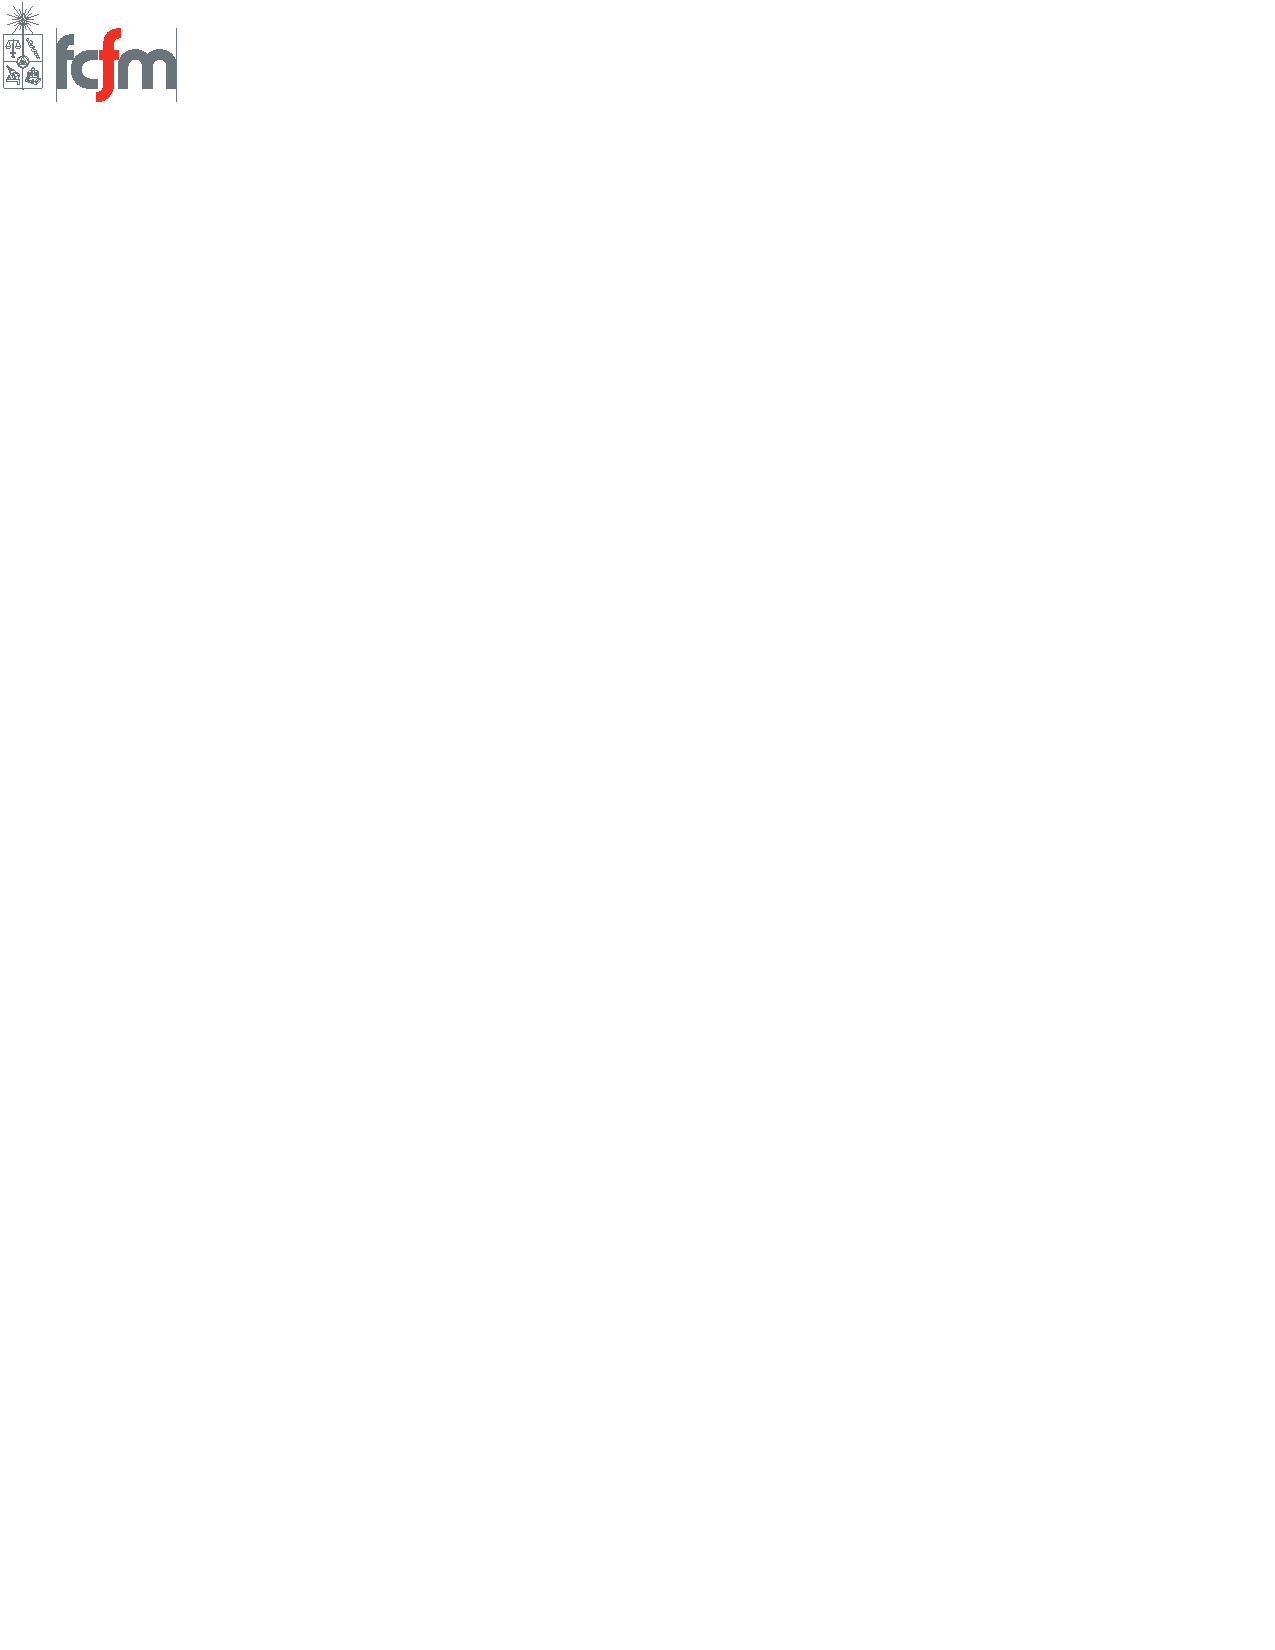
\includegraphics[scale=1.25]{2020-1/Imágenes/logo/fcfm2.pdf}}
\end{picture}

\begin{center}
	\LARGE \bf Ejercicio \#1 \\
\end{center}

\vspace{-1cm}
\begin{enumerate}\setlength{\itemsep}{0.4cm}

\rfoot[]{pág. \thepage}

\item[]

\item Se tiene el siguiente gráfico que representa el movimiento de una partícula a lo largo de un eje rectilíneo:\\
    \begin{figure}[h!]
        \centering
        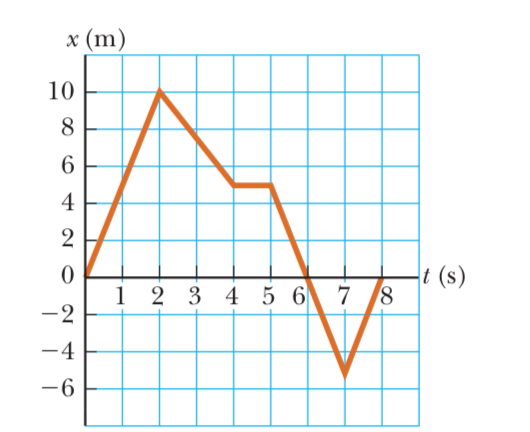
\includegraphics[]{2020-1/Imágenes/ejercicios/Ejercicio_1_p1.png}
    \end{figure}
\\ La escuela le pide a usted como experto en cinematica en 1-D que encuentre:
\begin{enumerate}
    \item La velocidad media, o promedio, en los siguientes intervalos de tiempo:
        \begin{enumerate}
            \item 0s a 2s
            \item 0s a 4s
            \item 2s a 4s
            \item 4s a 7s 
            \item 0s a 8s
        \end{enumerate}
    \item Calcule la velocidad instantánea a los:
        \begin{enumerate}
            \item t= 1 s
            \item t= 3 s
            \item t= 4,5 s
            \item t= 7,5 s
        \end{enumerate}
    \item ¿ Cuál es la velocidad instantánea en t=2,t=4,t=5,t=7? ¿Es la representación del gráfico físicamente posible ?
\end{enumerate}

\end{enumerate}
\end{document}